\section*{Introduction du chapitre \thechapter}

Nous pr�sentons maintenant une application de Imogene au cas de la
diff�renciation des trichomes, ou poils, chez la Drosophile. Plusieurs motifs
ont �t� g�n�r�s � partir de $14$ CRMs connus pour r�guler le processus de
diff�renciation des trichomes. Parmi les motifs g�n�r�s, deux d'entre eux ont
montr� une meilleure capacit� � distinguer les CRMs positifs de l'ensemble
d'apprentissage de CRMs n�gatifs. Le crit�re de distinction est bas� sur
l'optimisation de Pareto, caract�risant la satisfaction de plusieurs
contraintes � la fois. Dans notre cas, les contraintes sont de maximiser le
nombre de CRMs positifs trouv�s par les motifs (maximisation de la sensibilit�)
tout en minimisant le nombre de faux positifs (maximisation de la sp�cificit�).
Ces crit�res d�finissent une fronti�re de Pareto de motifs optimum. En variant
les diff�rents param�tres de Imogene, nous avons trouv� deux motifs sur la
fronti�re de Pareto. Parmi les deux motifs, l'un d'eux (\og svbf7 \fg)
correspond au r�gulateur ma�tre du processus de diff�renciation des trichomes,
et l'autre (\og blue motif\fg) est un motif nouveau. L'importance des deux
motifs pour la r�gulation est montr�e par mutagen�se. Par ailleurs, ces motifs
permettent de distinguer des \chipseq pour \textit{svb} li�s � une r�gulation
(dont le g�ne le plus proche subit une perte d'expression lors du KO de
\textit{svb}) des \chipseq ne l'�tant pas. Ce travail montre donc un exemple de
la possibilit� d'utiliser Imogene sur sun un petit ensemble (ici $14$ CRMs) de
donn�es biologiques fonctionnelles pour d�tecter des motifs nouveaux et
fonctionnels.



%%%%%%%%%%%%%%%%%%%%%%%%%%%%%%%%%%%%%%%%%%%%%%%%%%%%%%%%%%%%%%%%%%%%%%%%%%%%%%%%%%%%%%%%%%%%%%%%%%%	%%%%%%%%%%%%%%%%%%%%%%%%%%%%%%%%%%%%%%%%%%%%%%%%%%%%%%%%%%%%%%%%%%%%%%%%%%%%%%%%%%%%%%%%%%%%%%%%%%%	
\newpage


\section{Article} 
\label{sec:article}

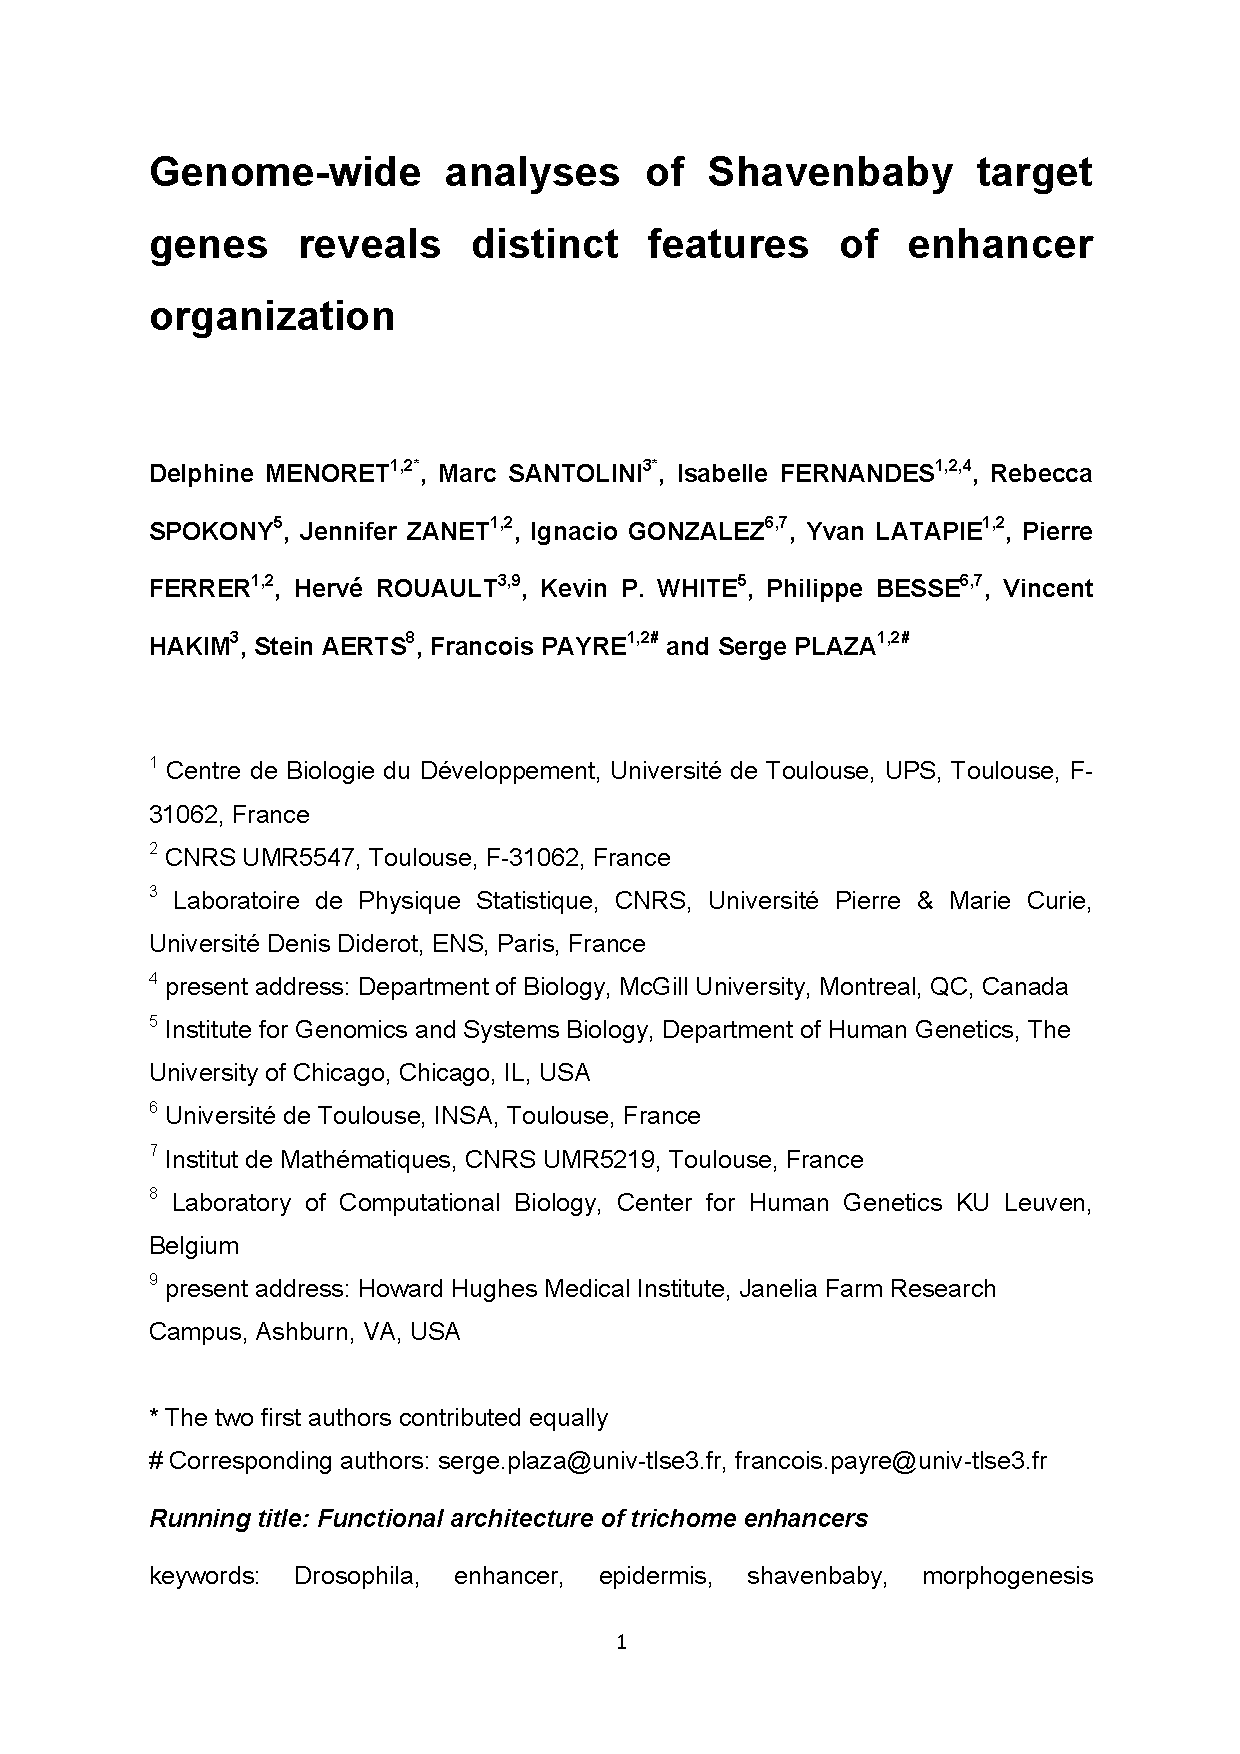
\includepdf[pages=-]{articles/trichomes-genomebiol/Menoret_et_al_GenBiol_revised.pdf}
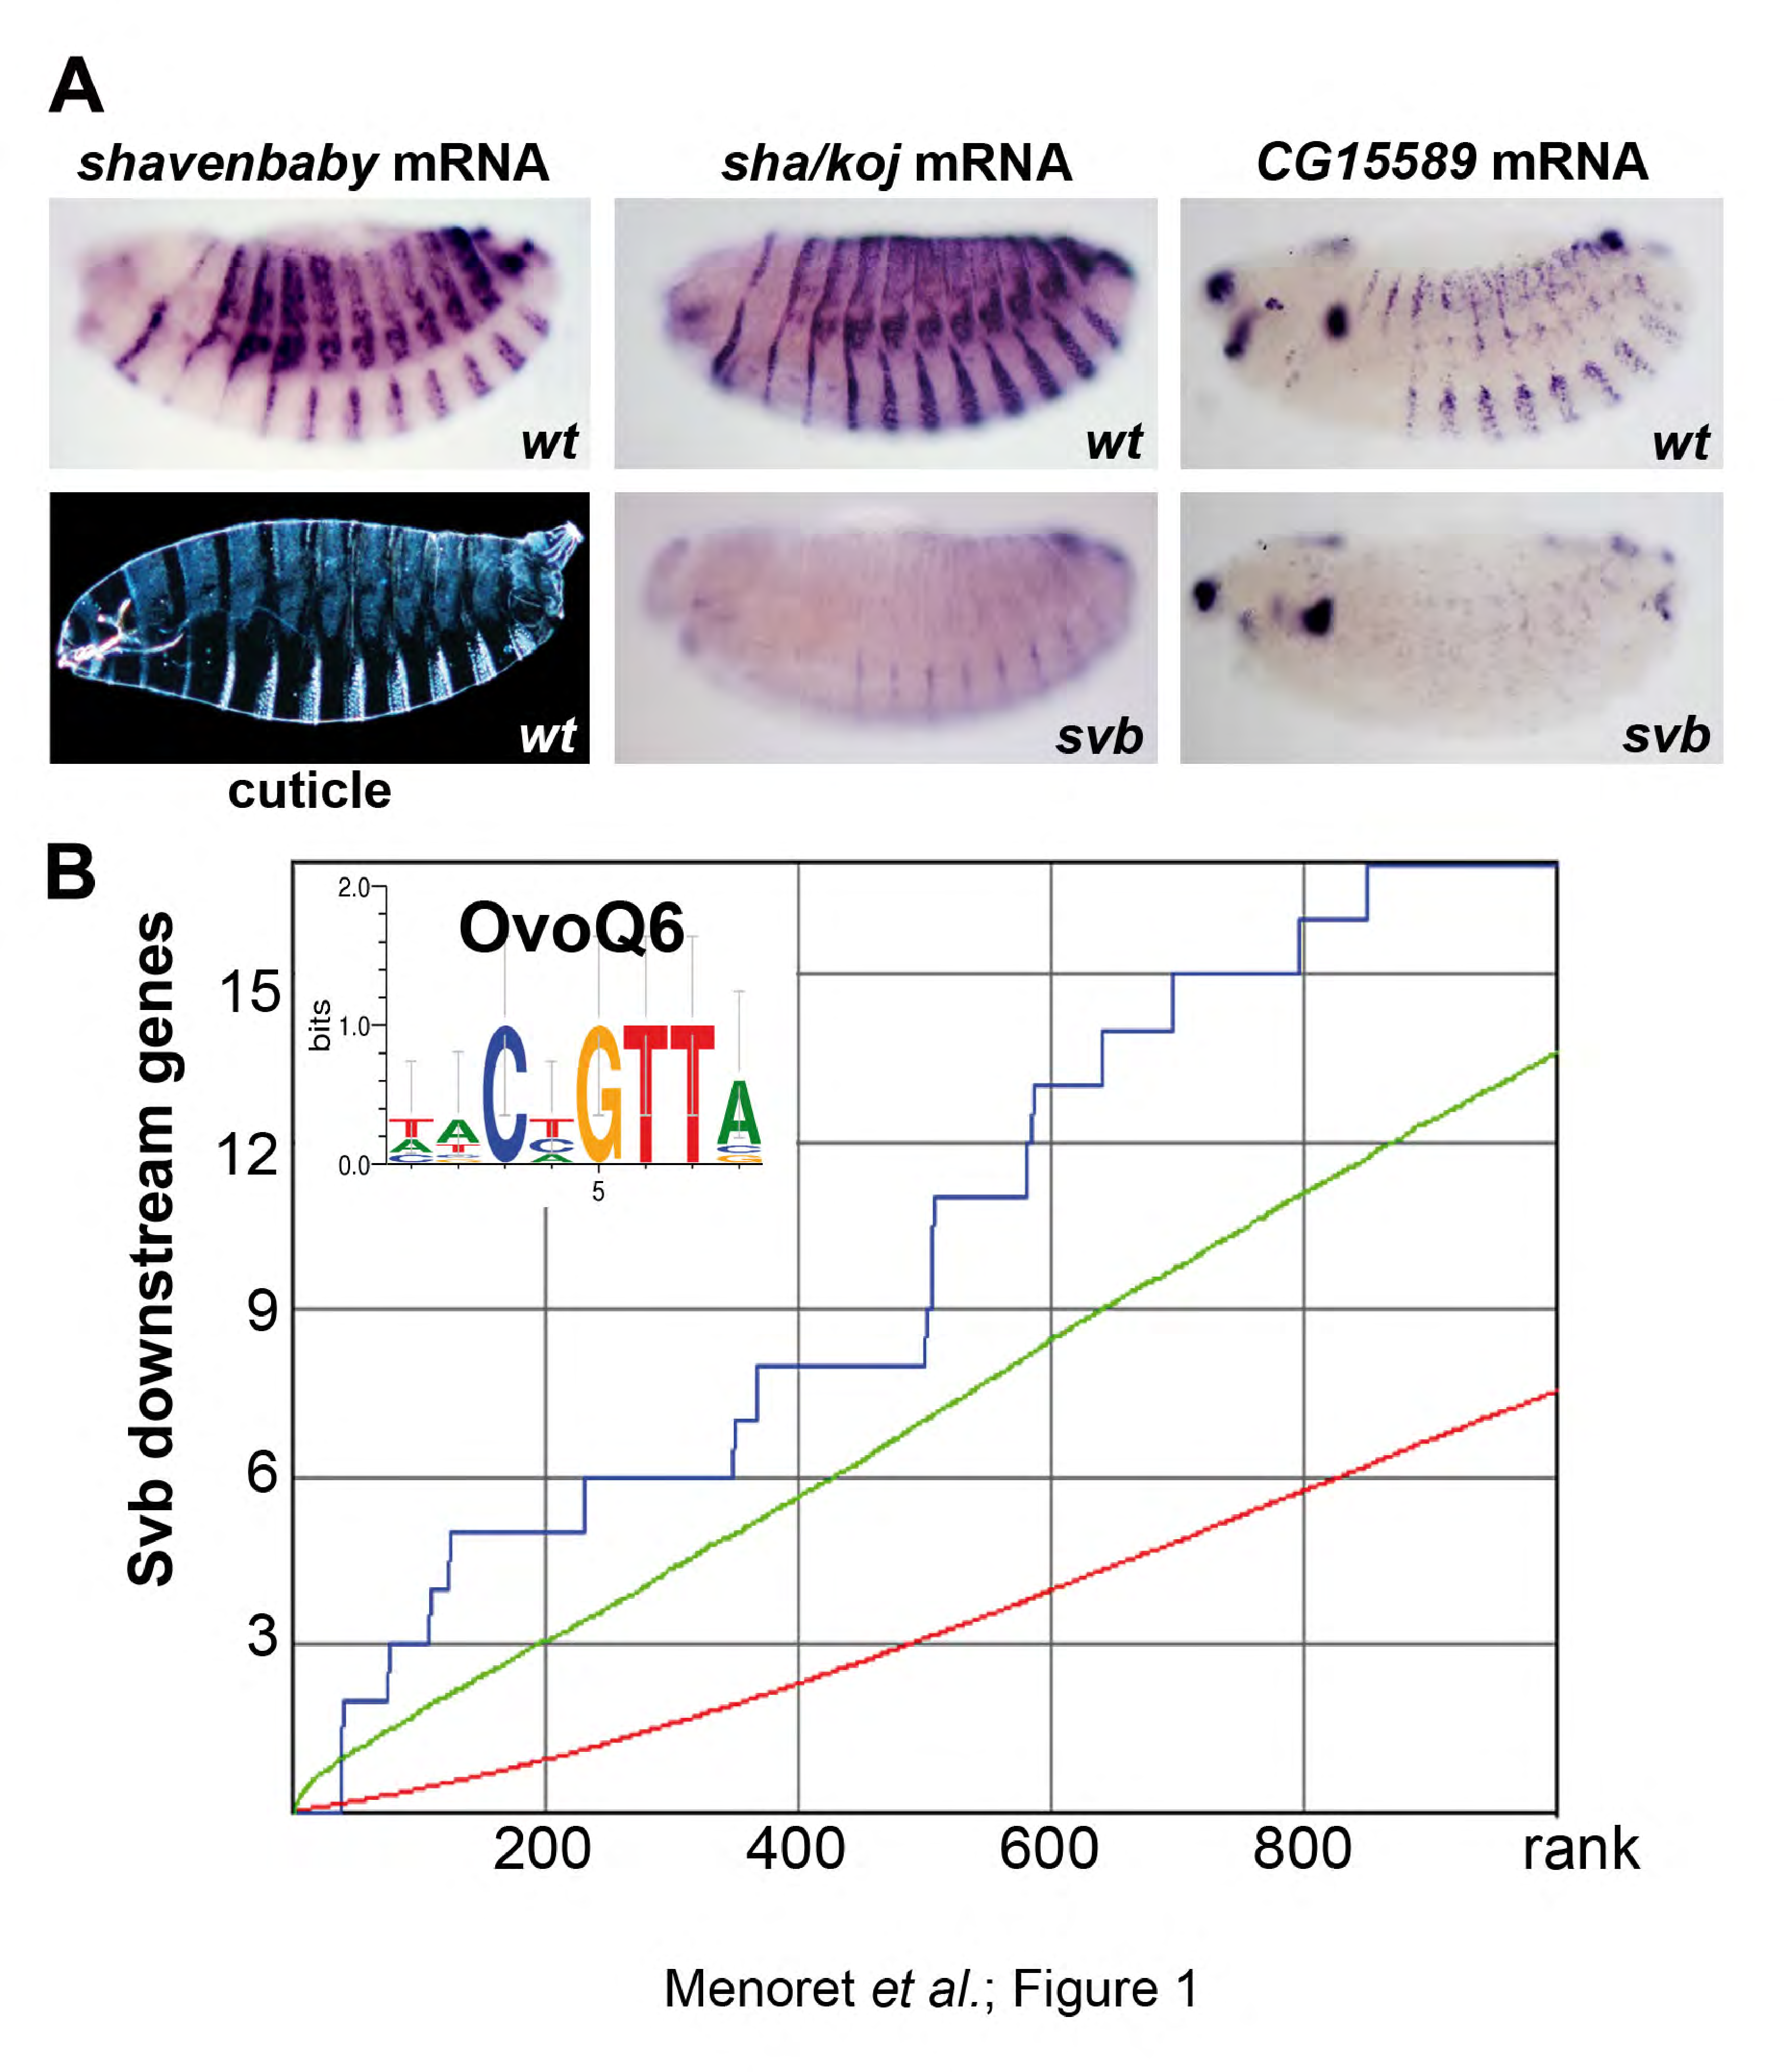
\includepdf[pages=-]{articles/trichomes-genomebiol/Figures_rev_S.pdf}
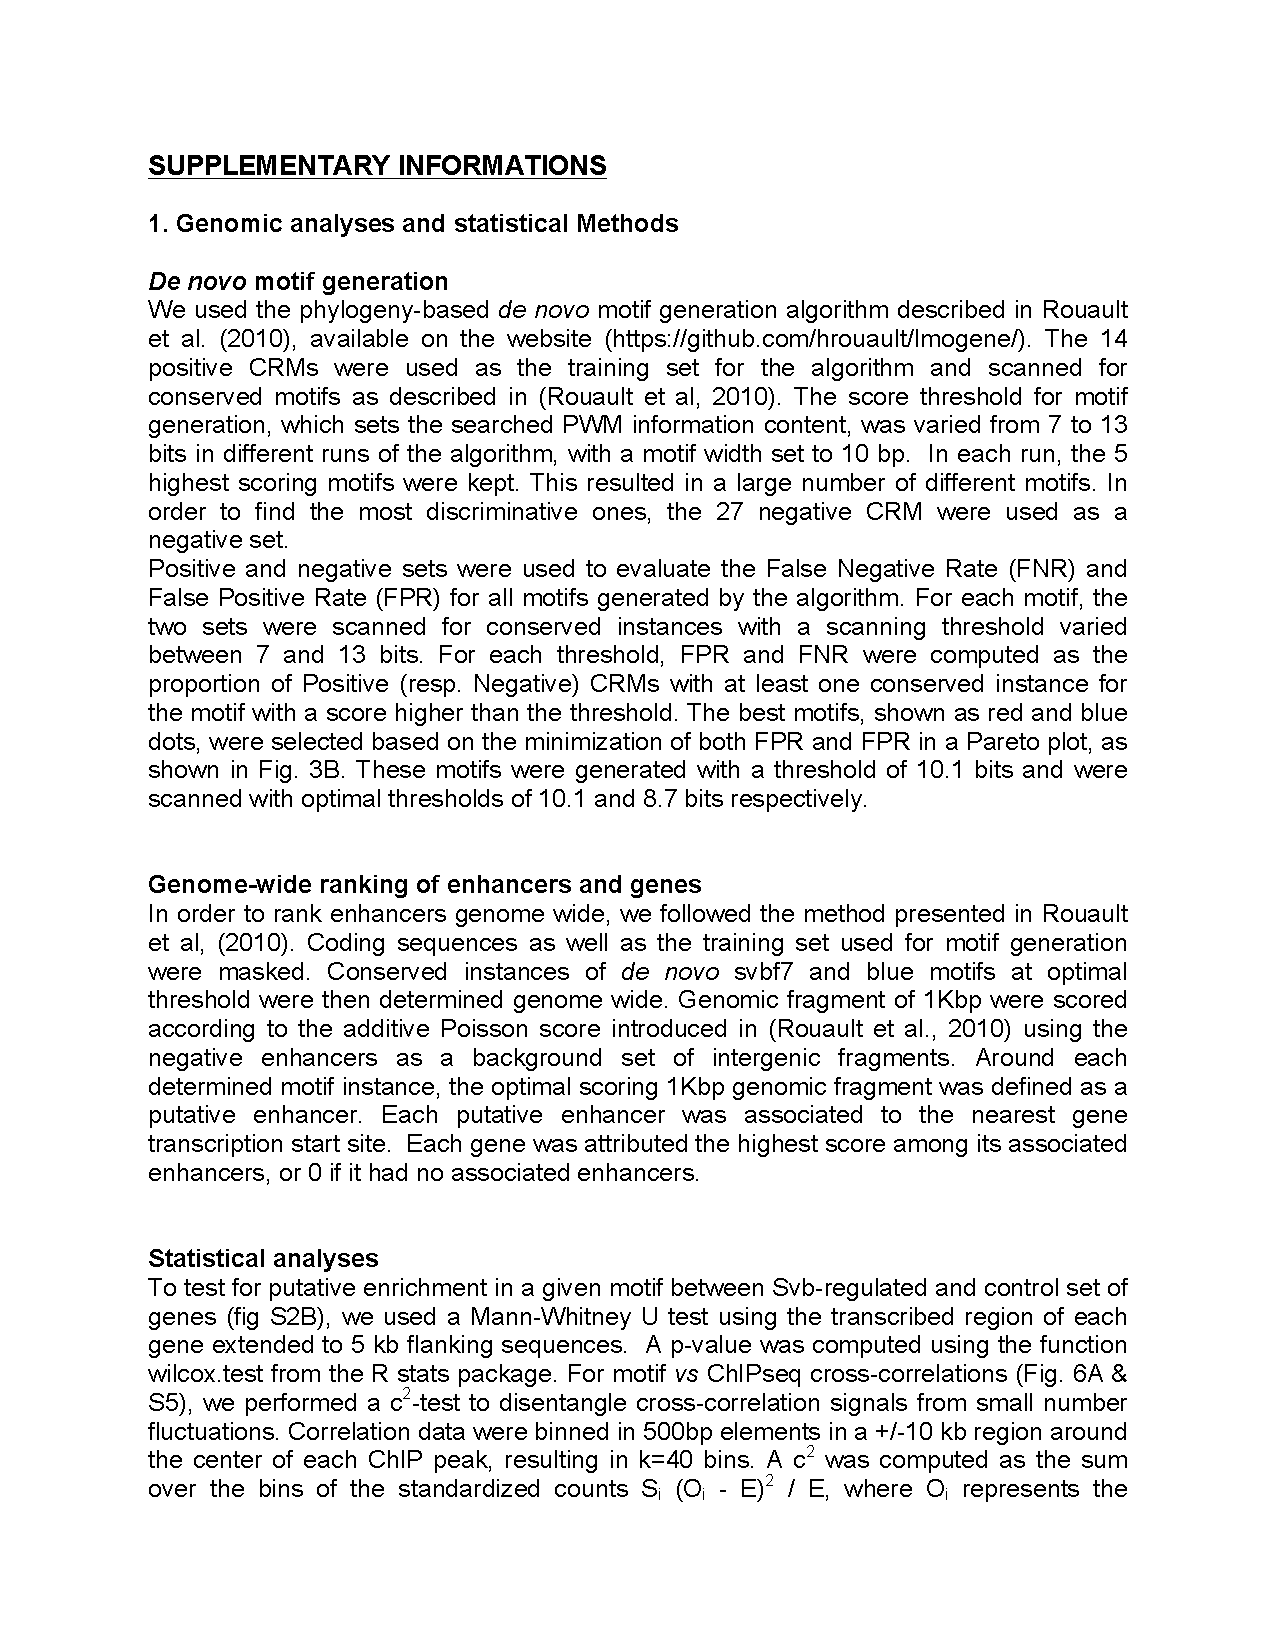
\includepdf[pages=-]{articles/trichomes-genomebiol/Menoret_SupInfos_revised.pdf}
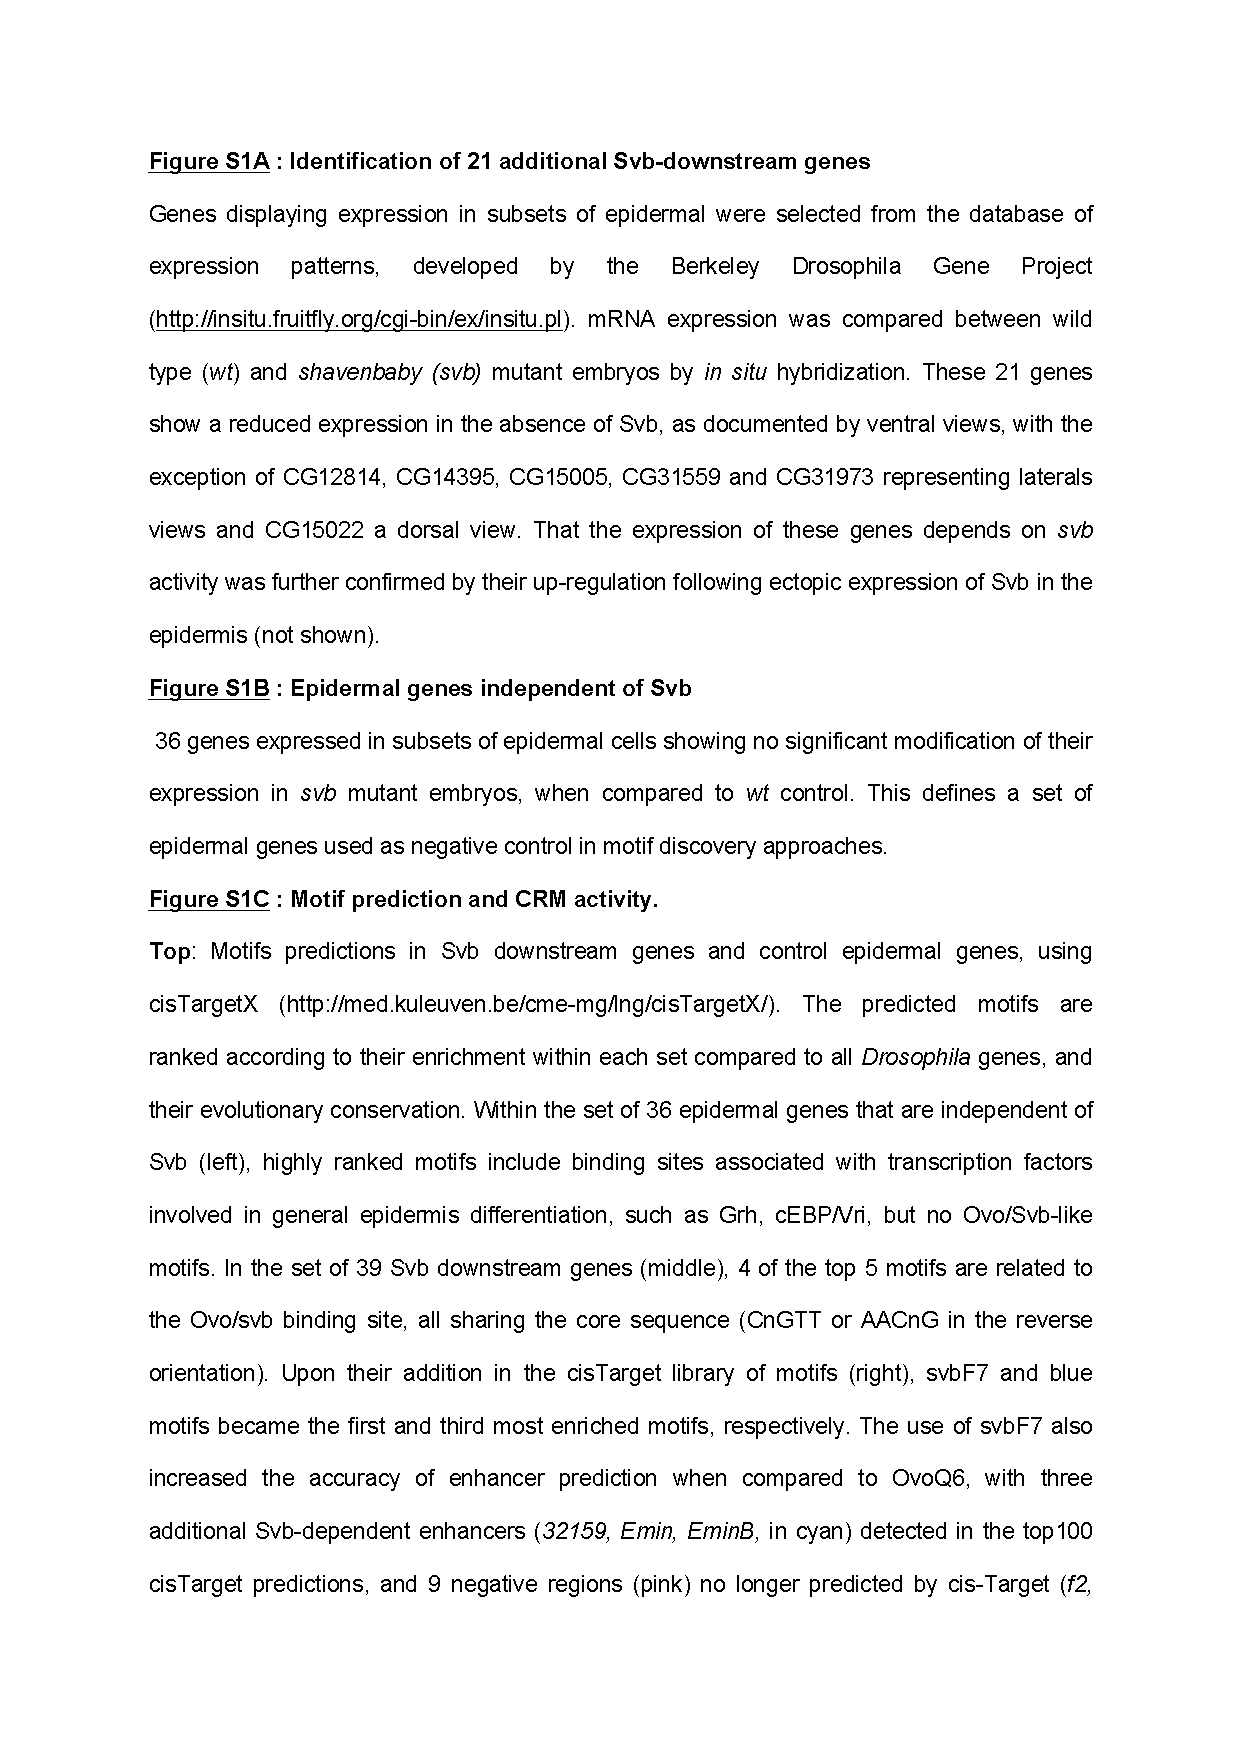
\includepdf[pages=-]{articles/trichomes-genomebiol/Menoret_et_al_FigSupLegend_revised.pdf}
\includepdf[pages=-]{articles/trichomes-genomebiol/FigSup_rev_S.pdf}
% section article (end)
			
%%%%%%%%%%%%%%%%%%%%%%%%%%%%%%%%%%%%%%%%%%%%%%%%%%%%%%%%%%%%%%%%%%%%%%%%%%%%%%%%%%%%%%%%%%%%%%%%%%%	%%%%%%%%%%%%%%%%%%%%%%%%%%%%%%%%%%%%%%%%%%%%%%%%%%%%%%%%%%%%%%%%%%%%%%%%%%%%%%%%%%%%%%%%%%%%%%%%%%%	
\newpage	
			
\section*{Conclusion du chapitre \thechapter}
